\section{Generaci\'on de Expresiones referenciales}

La generaci\'on de expresiones referenciales (GRE) {dado un contexto y un elemento
en ese contexto generar una expresi\'on gramaticalmente correcta en un lenguaje natural que representa \'unicamente el elemento {es una tarea b\'asica en lenguaje natural
generaci\'on, y una \'area de investigaci\'on activa (ver [4,5,6,20,8] entre otros). La mayor\'ia de
trabajo en esta \'area se centra en el problema de la determinaci\'on del contenido (es decir, encontrar una conjunto de propiedades que singulariza el objeto target de los restantes
objetos en el contexto) y deja la realizaci\'on real (es decir, que expresa un hecho
contenido como una expresi\'on gramaticalmente correcta) para tecnicas est\'andares.(excepto 16,21)
Sin embargo, a\'un no existe un acuerdo general sobre la representaci\'on b\'asica de
tanto la entrada y la salida del problema; esto se maneja mas bien de manera ad-hoc
por cada nueva propuesta.
Krahmer et al. [17] usan grafos dirigidos etiquetados en el contexto de este problema: los grafos son lo suficientemente abstractos para expresar un gran n\'umero de

dominios y hay muchos atractivos y algoritmos conocidos para tratar
con este tipo de estructuras. De hecho, no se trata de otra cosa que una representaci\'on alternativa de los modelos relacionales, usada t\'ipicamente para proporcionar sem\'antica a los lenguajes formales como el de primer orden y l\'ogicas de orden superior, l\'ogicas modales, etc.

''Incluso las valoraciones'' (esto no entendi...), los modelos b\'asicos de la l\'ogica proposicional, pueden ser vistos como un grafo de un solo punto etiquetado.
 No es de extra\~nar que son muy adecuadas para la tarea.
En este art\'iculo, nos ponemos del lado de [17] y usamos grafos etiquetados como entrada, pero sostenemos que una noci\'on importante se ha quedado fuera al tomar esta decisi\'on. Exactamente debido a su generalidad, los grafos no se definen por s\'i mismos, una unica noci\'on de igualdad. �Cu\'ando decimos que dos nodos en el grafo pueden o no pueden ser
referenciados de forma \'unica en t\'erminos de sus propiedades? Esta pregunta s\'olo tiene sentido una vez que ya hemos fijado un cierto nivel de expresividad el cual determina cuando dos grafos, o dos elementos en el mismo gr\'afico, son equivalentes.
La expresividad se puede formalizar usando las relaciones estructurales de los grafos (iso
morfismos, etc.) o, alternativamente, lenguajes l\'ogicos. Ambas formas se presentan
en [cap2], donde tambi\'en discutimos c\'omo arreglar la noci\'on de impacto de expresividad en el n\'umero de casos que el problema GRE tiene soluci\'on; la complejidad computacional de los algoritmos GRE involucrados; y la complejidad computacional del problema de la realizaci\'on. Luego investigamos el problema GRE en t\'erminos de diferentes 
nociones de expresividad. Primero exploramos en [cap3] c\'omo algoritmos conocidos de
l\'ogica computacional se puede aplicar a GRE. Esta es una sistematizaci\'on de la aproximacion en [cita 1], y somos capaces de responder a la pregunta de complejidad que quedaba abierta.
En [cap4] tomamos el camino opuesto: tomamos el conocido algoritmo de GRE-
de [cita 17], identificamos su expresividad subyacente y lo reescribimos en t\'erminos de otras l\'ogicas.
A continuaci\'on, mostramos en [cap5] que ambos enfoques se pueden combinar y finalmente discutimos en [cap6] el tama\~no de una RE con respecto a la expresividad empleada. Llegamos a la conclusi\'on en [cap7] con una breve discusi\'on y las perspectivas para el trabajo futuro.

\newcommand{\nDog}{\mathit{dog}\xspace}
\newcommand{\nCat}{\mathit{cat}\xspace}
\newcommand{\aSmall}{\mathit{small}\xspace}
\newcommand{\aSniffing}{\mathit{sniffs}\xspace}
\newcommand{\nBreed}{\mathit{beagle}\xspace}

\section{Mediendo el poder expresivor}\label{sec:technical}


Las estructuras relacionales son muy adecuadas para la representaci\'on de situaciones o escenas. La estructura relacional (tambi\'en llamado ''el modelo relacional'') es un conjunto no vac\'io de objetos -el dominio- junto con una colecci\'on de las relaciones, cada uno con una aridad fija.
Formalmente, asumimos un vocabulario fijo y finito (pero arbitrario) vocabulario de
s\'imbolos de relaci\'on n-aria (las constantes y s\'imbolos de funci\'ones pueden ser representados como relaciones de aridad adecuada). 
Un modelo relacional $\+M$ es una tupla 
$\tup{\Delta,\interp{\cdot}}$ donde $\Delta$ es un conjunto no vac\'io, y
$\interp{\cdot}$ es una funci\'on de interpretaci\'on, esto es,
$\interp{r} \subseteq \Delta^n$ para todo s\'imbolo de relaci\'on $n$-aria tal que
$r$ est\'a en el vocabulario. Decimos que $\+M$ es \emph{finite} cuando
$\Delta$ es finito.  El \emph{tama\~no} de un modelo $\+M$ es la suma
$\#\Delta + \#\interp{\cdot}$, donde $\#\Delta$ es la cardinalidad
de $\Delta$ y $\#\interp{\cdot}$ es la suma de los tama\~nos de todas las
relaciones en $\interp{\cdot}$.

La Figura~\ref{fig:cat-dog-1} abajo muestra como nosotros podemos representar una escene
as un modelo relacional. Intuitivamente, $a$, $b$ y $d$ son dogs, mientras que 
$c$ y $e$ are cats;  $d$ es un small beagle;
 $b$ y $c$ son tambi\'en small.
 Nosotros leemos $\aSniffing(d,e)$ como ``{\em $d$ is sniffing $e$}''.

 \begin{figure}
 \begin{center}
 \begin{tabular}{rcl}
$\Delta$               & = & $\cset{a,b,c,d,e}$\\
$\interp{\nDog}$      & = & $\cset{a,b,d}$\\
$\interp{\nCat}$      & = & $\cset{c,e}$\\
$\interp{\nBreed}$    & = & $\cset{d}$\\
$\interp{\aSmall}$    & = & $\cset{b,c,d}$\\
$\interp{\aSniffing}$ & = & $\cset{(a,a),(b,a),(c,b),(d,e),(e,d)}$
 \end{tabular}
\begin{picture}(120,50)
\put(0,-50){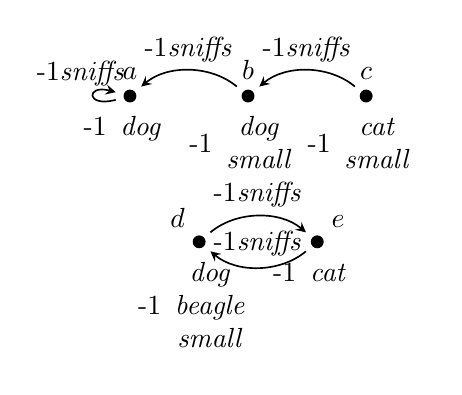
\begin{tikzpicture}
  [
    n/.style={circle,fill,draw,inner sep=1.5pt,node distance=1.5cm},
    aSniffing/.style={->, >=stealth, semithick, shorten <= 3pt, shorten >= 3pt},
  ]
 \node[n,label=above:$a$,label=below:{\relsize{-1}$\begin{array}{c}\nDog\end{array}$}] (a) {};

 \node[n,label=above:$b$,label=below:{\relsize{-1}$\begin{array}{c}\nDog\\ \aSmall \end{array}$}, right of=a] (b) {};

 \node[n,label=above:$c$,label=below:{\relsize{-1}$\begin{array}{c}\nCat\\ \aSmall\end{array}$}, right of=b] (c) {};

 \node[n,label=above left:$d$,label=below:{\relsize{-1}$\begin{array}{c}\nDog\\ \nBreed\\  \aSmall \end{array}$}, below of=a,xshift=25pt,yshift=-10pt] (d) {};

 \node[n,label=above right:$e$,,label=below:{\relsize{-1}$\begin{array}{c}\nCat\end{array}$},right of=d] (e) {};

 \draw [aSniffing,loop left] (a) to node[above,xshift=-5pt]{\relsize{-1}$\aSniffing$} (a);

 \draw [aSniffing,bend right=40] (b) to node[auto,swap]{\relsize{-1}$\aSniffing$} (a);

 \draw [aSniffing,bend right=40] (c) to node[auto,swap]{\relsize{-1}$\aSniffing$} (b);

 \draw[aSniffing, bend left=40] (d) to node[auto]{\relsize{-1}$\aSniffing$} (e);
 \draw[aSniffing, bend left=40] (e) to node[auto,swap]{\relsize{-1}$\aSniffing$} (d);

 \end{tikzpicture}}
 \end{picture}

 \end{center}
 \caption{Representaci\'on de escenas de Graph $\+S$.\label{fig:cat-dog-1}}
 \end{figure}


Los languajes logicas son \'utiles para la tarea (formalmente) \emph{describiendo}
elementos de una estructura relational. Consider, por ejemplo, el lenguaje clasico
de l\'ogica de primer-orden (con igualdad), \FOL, dado por:
$$
  \top \mid x_i \not\approx x_j \mid  r (\bar x) \mid \lnot \gamma \mid \gamma \land \gamma' \mid \exists x_i . \gamma
$$
%
donde $\gamma,\gamma' \in \FOL$,
$r$ es un s\'imbolo de relaci\'on $n$-ario y $\bar x$ es un $n$-tuple de variables.
Como es usual, $\gamma \lor \gamma'$ y $\forall x . \gamma$ son las versiones cortas de
$\lnot(\lnot\gamma \land \lnot\gamma')$ y $\lnot\exists x . \lnot\gamma$, respectivamente.
Formulas of the form $\top$, $x_i \not\approx x_j$ and $r(\bar
x)$ son llamados \emph{atomos}.%
  \footnote{%
    Por razones t\'ecnicas, incluimos el s\'imbolo de desigualdad symbol $\not \approx$ como
    primitivo.  Igualdad puede ser definido usando negaci\'on.
  }
Dado un modelo relacional $\+M = \tup{\Delta,\interp{\cdot}}$ y una
f\'ormula $\gamma$ con variables libres%
\footnote{%
    W.l.o.g.\ asumimos que no aparecen variable en ambos, libres y ligadas, que una variable no esta ligada 2 veces,
    y que el \'indice de las variables crece en la f\'ormula de izquierda a derecha.%
}
entre $x_1\ldots x_n$, inductivamente definimos la \emph{extensi\'on} o
\emph{interpretaci\'on} de $\gamma$ como el conjunto de $n$-tuplas
 $\interp{\gamma}^n \subseteq \Delta^n$ que satisface:

\begin{center}
\begin{tabular}{rcl@{\hspace{1cm}}rcl}
$\interp{\top}^n$ &$=$& $\Delta^n$
&
$\interp{x_i \not\approx x_j}^n$ &$=$& $\cset{\bar{a} \mid \bar{a} \,{\in}\, \Delta^n, a_i \neq a_j}$
\\
$\interp{\lnot\delta}^n$ &$=$& $\Delta^n \setminus \interp{\delta}^n$
&
$\interp{r (x_{i_1} \ldots x_{i_k})}^n$ & $=$&$\cset{\bar{a} \mid \bar{a} \,{\in}\, \Delta^n, (a_{i_1} \ldots a_{i_k}) {\in} \interp{r}}$
\\
$\interp{\delta \land \theta}^n$ &$=$& $\interp{\delta}^n \cap \interp{\theta}^n$
&
$\interp{\exists x_{l}.\delta}^n$ &$=$& $\cset{\bar a \mid \bar a  e  \in \interp{\delta'}^{n+1}\ \text{for some $e$}}$
\end{tabular}
\end{center}
%
donde $1 \le i,j, i_1, \ldots, i_k \le n$, $\bar{a} = (a_1\ldots
a_n)$, $\bar{a}e = (a_1\ldots a_n,e)$ y $\delta'$ son
obtenidos reeplazando todas las ocurrencias de $x_l$ en $\delta$ por
$x_{n+1}$. Cuando la cardinalidad de las tuplas involucradas en el contexto es conocida 
escribiremos $\interp{\gamma}$ en lugar de
$\interp{\gamma}^n$.

Con una sintaxis y sem\'antica de un lenguaje en mente, podemos formalmente definir el problema de L-GRE para un conjunto target de elementos T (lejeramente adaptaremos la definici\'on en ~\cite{AKS08}):

\medskip
\noindent
{\small
\begin{center}
\begin{tabular}{ll} \hline
\multicolumn{2}{l}{
\textsc{Problema $\gL$-GRE }}\\ \hline
\ \ Input: & a model $\gM=\tup{\Delta,\interp{\cdot}}$ and a nonempty target  set $T \subseteq \Delta$.\\
\ \ Output: & a formula $\varphi \in \gL$ such that
$\interp{\varphi} = T$ if it exists, and $\bot$ otherwise.\\ \hline
\end{tabular}
\end{center}}
Cuando el output es no $\bot$, decimos que $\phi$ es una
\emph{$\+L$-referring expression ($\+L$-RE) para $T$ en $\+M$}.
Simply put then, el output de el problema $\+L$-GRE es una f\'ormula de
$\+L$ cuya interpretaci\'on en el modelo de input es el conjunto target, si
tal f\'ormula existe.  Esta definici\'on aplica incluso a la GRE para
objetos  de el dominio teniendo un conjunto singleton como target.

Mediante el uso de f\'ormulas con n variables libres se podr\'ia extender esta defici\'on para
describir relaciones n-arias; pero aqu\'i s\'olo estamos interesados ??en la descripci\'on de subconjuntos de
el dominio. En realidad, limitaremos nuestra atenci\'on un poco m\'as:
Convenci\'on 1. S\'olo consideraremos modelos relacionales con s\'imbolos de relaciones unarias y binarias
 (es decir, grafos etiquetados ). Usaremos p para los s\'imbolo de relaci\'on unarios
 (y lo llamaremos una proposici\'on) y r para los s\'imbolos de relaciones binarios.
Esta convenci\'on captura los modelos habituales de inter\'es al describir escenas como
el presentado en la Figura ~\ref{fig:cat-dog-1}. Acomodando las relaciones de mayor aridad en nuestra
marco te\'orico es f\'acil, pero puede ser que una complejidad computacional? ect.

\subsection{Elecci\'on del lenguaje apropiado}\label{sec:choosinglanguage}

Dado un modelo M, podr\'ia haber un infinito n\'umero de f\'ormulas que de forma \'unica
describan un target (incluso f\'ormulas que no son l\'ogicamente equivalentes podr\'ian tener
la misma interpretaci\'on una vez al modelo este fijo). A pesar de tener la misma interpretaci\'on en M, ellos pueden ser muy diferentes con respecto a otros par\'ametros.
Como es bien conocido en la comunidad generaci\'on de texto automatizado, diferentes
realizaciones del mismo contenido podr\'ian dar lugar a expresiones referenciales que son m\'as o menos
apropiadas en el contexto dado. Aunque, como hemos mencionado en la introducci\'on,
s\'olo nos ocuparemos de la parte determinaci\'on del contenido (y no de la parte de realizaci\'on) del problema GRE, argumentamos que la generaci\'on de contenido usando lenguajes con diferente poder expresivo puede tener un impacto en la estapa posterior
de generaci\'on de superficie (surface realization, realizaci\'on sint\'actica... pero es mucho m\'as que eso... ).


Consideremos de nuevo la escena en la Figura~\ref{fig:cat-dog-1}. F\'ormulas

$\gamma_1$--$\gamma_4$ mostradas en la Tabla~\ref{tab:gammas}
son todas de tal manera que $\gamma_i$ \'unicamente describe a $b$
(es decir, $\interp{\gamma_i} = \cset{b}$) en el modelo $\+S$.
Podr\'ia decirse que, $\gamma_1$ puede ser f\'acilmente realizada como \emph{``the small dog
that sniffs a dog''}. Sint\'acticamente, $\gamma_1$ es caracterizada como una f\'ormula positiva, conjuntiva, existencial (es decir, no contiene negaci\'on y s\'olo utiliza la conjunci\'on y cuantificaci\'on existencial). Expresiones
con estas caracter\'isticas son, por mucho, las m\'as encontradas en los corpus de ER
como los recopilados en~\cite{viet:algo06,deem:buil06,dale:refe09}. La f\'ormula $\gamma_2$, por otro lado, contiene negaci\'on,
disyunci\'on y cuantificaci\'on universal. Podr\'ia realizarse como \emph{``the small dog that
only sniffs things that are not cats''} lo cual suena poco natural. 

Incluso un peque\~no cambio en la f\'ormula $\gamma_2$ la hace m\'as aceptable:
reescribirla usando $\exists$, $\lnot$, y $\land$ para obtener
\emph{``the small dog that is not sniffing a cat''}. Similarmente,
 $\gamma_3$ y $\gamma_4$ son computacionalmente m\'as dificiles de realizar que 
 $\gamma_1$: $\gamma_3$ contiene desigualdad (\emph{``the dog sniffing another dog''}), mientras que el objeto cuantificado aparece en posici\'on del primer argumento en la relaci\'on binaria en $\gamma_4$ (\emph{``the dog that is sniffed by a small cat''}).


Resumiendo, podemos asegurar, ya durante la fase de determinaci\'on de contenido,
ciertas propiedades de la expresi\'on referencial generada prestando atenci\'on a
el lenguaje formal utilizado en la representaci\'on. Y podemos hacer esto, incluso antes
teniendo en cuenta otros aspectos ling�\'isticos fundamentales que se asegurar\'a de
realizaci\'on preferible, como la prominencia, la capacidad cognitiva del oyente (puede que
reconocer un beagle de otro tipo de perro?), etc.
Como ejemplo concreto, vamos FO? ser el fragmento del FO-f\'ormulas donde el
 como el conjunto de n-tuplas
\begin{table}
$$
\begin{array}{cl}
 \gamma_1: & \nDog(x) \land \aSmall(x) \land
   \exists y . (\aSniffing(x,y) \land \nDog(y))\\[3pt]
  %
  \gamma_2: & \nDog(x) \land \aSmall(x) \land
  \forall y . (\neg \nCat(y) \lor \neg \aSniffing(x,y))\\[3pt]
  %
  \gamma_3: & \nDog(x) \land
  \exists y . (x \not\approx y \land \nDog(y)  \land \aSniffing(x,y))\\[3pt]
  %
  \gamma_4: & \nDog(x) \land
  \exists y . (\nCat(y) \land \aSmall(y) \land \aSniffing(y,x))
  %
 \end{array}
$$
\caption{Alternative descriptions for object $b$ in the model shown in Figure~\ref{fig:cat-dog-1}.}\label{tab:gammas}
\end{table}

reemplazando todas las ocurrencias de xl en? por xn + 1. Cuando la cardinalidad de las tuplas
involucrados se conoce a partir del contexto nos limitaremos a escribir jj
jj lugar de jj
JJN.
Con una sintaxis del lenguaje y la sem\'antica en su lugar, ahora podemos formalmente de ne
el problema de la L-GRE para un objetivo conjunto de elementos de T (que poco adaptar el
de definici\'on en [1]):
L-GRE Problema
Entrada: un modelo M = h ?; jj? JJI y un objetivo conjunto no vac\'io T? ?.
Salida: una f\'ormula '2 L tal que jj'jj = T si es que existe, y? de otra manera.
Cuando la salida no es?, Se dice que "es un L-refiri\'endose expresi\'on (L-RE)
para T en M. En pocas palabras a continuaci\'on, la salida del problema L-GRE es una f\'ormula
de L cuya interpretaci\'on en el modelo de entrada es el conjunto de destino, si tal f\'ormula
existe. Esta definici\'on de aplica tambi\'en a la GRE para los objetos del dominio por
teniendo un conjunto unitario fijado como objetivo.
6 Por razones t\'ecnicas, que incluyen el s\'imbolo de desigualdad 6? tan primitivo. Igualdad puede
ser de nido mediante la negaci\'on.
7 W.l.o.g. suponemos que ninguna variable aparece tanto libre y unida, que ninguna variable
est\'a unido dos veces, y que el \'indice de variables ligadas en una f\'ormula aumenta desde
de izquierda a derecha.

El uso de la l\'ogica en la Generaci\'on del Refiri\'endose Expresiones 5

1: Perro (x) ^ peque\~na (x) ^ 9y: (�sni s (x, y) ^ perro (y))

2: Perro (x) ^ peque\~na (x) ^ 8y :(: Gato (y) _:? Sni s (x, y))

3: Perro (x) ^ 9y: (x 6 y ^ perro (y) ^ sni s (x, y)??)

4: Perro (x) ^ 9y: (�gato (y) ^ peque\~na (y) ^ sni s (y; x))
Tabla 1. Descripciones alternativas para el objeto b en el modelo muestran en la Figura 1.
restringiendo la determinaci\'on del contenido de FO?, nos aseguramos de que f\'ormulas como
2 lo har\'a
no ser generado. Si prohibimos 6? de la lengua,
3 se opongan.
El hecho de que el lenguaje de representaci\'on utilizado tiene un impacto sobre el contenido
determinaci\'on es obvio, pero no ha recibido la atenci\'on que merece. Son-
ces et al. [1] utilizar di? Descripci\'on Erent l\'ogicas (una familia de lenguajes formales utilizado
en representaci\'on del conocimiento, ver [2]) para clasificar y dar un marco formal para
trabajo previo sobre GRE. Vamos a presentar r\'apidamente algunas de estas lenguas como nosotros
se menciona en las secciones futuras. Usando l\'ogicas descriptivas en lugar de
Fragmentos FO es s\'olo una cuesti\'on de notaci\'on, como la mayor\'ia de l\'ogicas descriptivas se pueden ver
fragmentos como impl\'icitas de FO. Por ejemplo, el lenguaje de la descripci\'on l\'ogica
ALC, sint\'acticamente de ne como el conjunto de f\'ormulas,
> J p j:
 j
 ^
0 j 9r:

(donde p es un s\'imbolo proposicional, ra s\'imbolo relacional binario, y
;
0 2
ALC) corresponde a un fragmento sint\'actico de FO sin 6 ?, como se muestra por la
traducci\'on est\'andar x:
? xi (>) =>? xi (
1 ^
2) =? Xi (
1) ^? Xi (
2)
? xi (p) = p (xi) xi (9r?:
) = 9xi + 1:? (R (xi; xi + 1) ^ xi + 1 (
))
? xi (:
) =:? Xi (
)
En efecto, dado un modelo relacional M, la extensi\'on de una f\'ormula ALC '
en M coincide exactamente con la extensi\'on de? x1 (') (v\'ease, por ejemplo, [2]). Gracias
a este resultado, para cualquier f\'ormula "de ALC y sus sublenguajes podemos de nir
jj'jj = jj? x1 (') jj. Volviendo a nuestro ejemplo anterior, mediante la restricci\'on de contenido
generaci\'on en f\'ormulas ALC (o equivalentemente, el fragmento correspondiente de FO)
evitar\'iamos f\'ormulas como
3 (sin igualdad) y
4 (aparece cuanti elemento ed
siempre en segunda posici\'on de argumento).
Generaci\'on se discute en [1], en t\'erminos de di? Descripci\'on Erent l\'ogicas como ALC
y EL (ALC sin negaci\'on). Vamos a ampliar los resultados en ese papel, con-
Sidering por ejemplo EL + (ALC con la negaci\'on permite s\'olo frente a unario
las relaciones), pero, en general, nos tomamos un enfoque te\'orico modelo y argumentan
que la cuesti\'on principal no es si se debe utilizar uno u otro (descripci\'on
ci\'on) l\'ogica para la generaci\'on de contenidos, sino que son el di sem\'antica? cias
se preocupa. Esto determina el formalismo l\'ogico requerido sino tambi\'en impactos
tanto en la determinaci\'on del contenido y los problemas de realizaci\'on superficie. Cada
lenguaje l\'ogico puede ser visto como un compromiso entre la expresividad, realiz-
capacidad y complejidad computacional. La selecci\'on apropiada para un particular,
Tarea GRE debe depender del contexto real.

2.2 De ning Igualdad
Intuitivamente, dado un lenguaje l\'ogico L decimos que un objeto u en un modelo M1 es
similar en L a un objeto v en un modelo M2 siempre todo L-f\'ormulas satis ed por
u tambi\'en se Satis ed por v Formalmente, vamos = M1 h 1.?; jj? jj1i y M2 = h 2?; jj? jj2i ser
dos modelos relacionales con u 2 1 y v 2 2?; seguimos la terminolog\'ia de [1]
y decir que u es-L similar a v (notaci\'on u L v) siempre que u 2 jj
JJ1 implica
v 2 jj
JJ2, para cada
 2 L. Es f\'acil demostrar que la L-similitud es re
reflexiva para todos
L, y sim\'etrico para los idiomas que contienen negaci\'on.
Observe que la L-similitud captura la noci\'on de 'capacidad identificadas en L'. Si nosotros
tomar M1 y M2 a ser del mismo modelo, a continuaci\'on, un objeto u en el modelo puede
carse \'unica identificaci\'on usando L si no hay ning\'un objeto v di? Erent de u tal que
u L v. En otras palabras, si hay dos objetos U y V en un modelo M tal que
u L v, entonces el problema L-GRE con entrada de M y destino T = fug no lo har\'a
\'exito ya que para todas las f\'ormulas
 2 L tenemos fu; vg? jj
jj 6 = fug.
La noci\'on de L-similitud entonces, nos da una manija en el problema L-GRE.
Por otra parte, podemos reformular esta de nici\'on de una manera estructural, por lo que no lo hacemos
que considerar en muchos L-f\'ormulas infinitamente decidir si u es-L similar a
v. Podemos reinterpretar L-similitud en t\'erminos de nociones de teor\'ia de modelos est\'andar
como isomorfismos o bisimulations que describen las propiedades estructurales de la
modelo, en lugar. Dados dos modelos h 1?; ? jj1i jj yh 2?; jj? jj2i, considere lo siguiente
propiedades de una relaci\'on binaria? ? ? 1? ? 2 (cf. Convenci\'on 1):
atomL:? Si u1 u2, entonces u1 2 jjpjj1) u2 2 jjpjj2
atomR:? Si u1 u2, entonces u2 2 jjpjj2) u1 2 jjpjj1
? Rell: Si u1 u2 y (u1; v1) 2 jjrjj1, entonces 9V2 st v1 v2 y? (u2; v2) 2 jjrjj2
? relR: Si u1 u2 y (u2, v2) 2 jjrjj2, entonces 9v1 st u1 v1 y? (u1; v1) 2 jjrjj1
injL:? es una funci\'on inyectiva (cuando restringido a su dominio)
injR:? ?1 es una funci\'on inyectiva (cuando restringe a su dominio)
Vamos a decir que una relaci\'on binaria no vac\'io? es un L-simulaci\'on cuando
satis ca las propiedades indicadas en la Tabla 2. Por ejemplo, un binario no vac\'io
relaci\'on que satisface it atomL y Rell es una simulaci\'on EL, como se indica en
la fila 4 de la Tabla 2. Por otra parte, vamos a decir que un objeto v L-simula u (notaci\'on
u L!
v) si existe una relaci\'on? satisfacer las propiedades correspondientes de tal manera que
u? . v El siguiente es un resultado fundamental teor\'ia de modelos:
Teorema 1. IfM1 h = 1?; ? jj jj1i andM2 = h 2?; jj? jj2i son modelos nite, u 2? 1
y v 2? 2, entonces u L v i? u L!
v (para L 2 FFO; FO?; ALC; EL; EL + g).

El uso de la l\'ogica en la Generaci\'on del Refiri\'endose Expresiones 7
Prueba. Algunos resultados son bien conocidos: FO!
es isomorfismo en grafos etiquetados [11];
ALC! corresponde a la noci\'on de bisimulaci\'on [3, Def. 2,16]; EL!
es una simulaci\'on como
de nida en [3, Def. 2.77]. Los casos restantes son simples variaciones de estos.
Por lo tanto, en la noche simulaciones models8 captura exactamente la noci\'on de simi-
laridad. El derecho a la implicaci\'on de la izquierda no se sostiene, en general, en los modelos nite.
L-simulaciones nos permiten determinar, en un correo? Manera reflexiva, cuando un objeto es
indistinguible de la otra en un modelo dado con respecto a L.
Por ejemplo, podemos comprobar que un EL!
b en el modelo de la Figura 1 (la relaci\'on
? = F (a; a); (a; b) g satis it atomL y Rell). Usando el teorema 1 concluimos
que no hay descripci\'on para EL-A, ya que para cualquier f\'ormula EL-
, Si un jj 2
jj, a continuaci\'on,
b 2 jj
jj. Observe que b 6EL!
una, ya que (aplicando de nuevo el teorema 1), b 2 jjsmall (x) jj
pero a = 2 jjsmall (x) jj. Si se opta por un lenguaje m\'as rico que EL, tales como EL +, uno
puede ser capaz de describir una: hay que tomar, por ejemplo, la f\'ormula de L + EL perro (x) ^: peque\~na (x).
Como veremos en la siguiente secci\'on, la simulaci\'on nos da un e? Ciente, com-
computacionalmente enfoque viable al problema de la L-GRE. Los algoritmos para calcular
muchos tipos de L-simulaciones son bien conocidos (v\'ease, [15,18,14,10]), y para muchos
idiomas (por ejemplo, ALC, ALC con las relaciones inversas, EL + y EL) corren en
tiempo polin\'omico (por otra parte, ning\'un algoritmo polin\'omico para FO o FO?-
la simulaci\'on se conoce e incluso la complejidad exacta del problema en estos casos
est\'a abierto [13]).
3 Establece GRE a trav\'es del simulador
En esta secci\'on vamos a discutir c\'omo resolver el problema de la L-GRE utilizando simulaci\'on.
Dado un modelo M = h ?; jj? JJI, el teorema 1 nos dice que si dos elementos distintos
u y v en? son tales que u L!
v entonces cada L-f\'ormula que es cierto en u es tambi\'en
cierto en v. Por lo tanto no existe una f\'ormula de L que puede referirse \'unicamente a la u. De esto
perspectiva, saber si el modelo contiene un elemento que es-L similares
pero distinta de u es equivalente a decidir si existe un L-RE para u.
Asumir un lenguaje fijo L y un modelo M. Supongamos que queremos hacer referencia a una
elemento u en el dominio del se\~nor Queremos calcular el conjunto simulador de
u de ne como simML
(u) = fv 2? �julio!
vg. Cuando el modelo M es claro a partir de la
contexto, acaba de escribir SIML. Si simML
(u) no es la fug singleton, la L-GRE
problema fug objetivo en M fallar\'a.
Un algoritmo se da en [14] para calcular SIMEL + (v) para cada elemento v de una
modelo nite dada M = h ?; jj? JJI en tiempo O (#? #jj? jj). Intuitivamente, este algo-
rithm de ne S (v) como un conjunto de candidatos para la simulaci\'on de v y sucesivamente re ne
mediante la eliminaci\'on de aquellas que no logran simular v. Al final, S (v) = SIMEL + (v).
El algoritmo se puede adaptar para calcular SIML para muchos otros idiomas L. En
particular, se puede utilizar para calcular SIMEL en tiempo polinomial que dar\'a
nosotros el algoritmo b\'asico para el establecimiento de un l\'imite superior a la complejidad de la
Problema EL-GRE {esto contestar una pregunta abierta de [1]. El pseudo-c\'odigo
se muestra en el algoritmo 1, que utiliza la siguiente notaci\'on: P es un conjunto fijo de

s\'imbolos de relaci\'on unarios, para v 2?, sea P (v) = fp 2 P 2 jv jjpjjg y dejar tambi\'en
sucr (v) = 2 fu? j (v; u) 2 jjrjjg para r un s\'imbolo de relaci\'on binaria.
Algoritmo 1: C\'alculo de EL-similitud
de entrada: un modelo finito M = h ?; jj? JJI
salida: 8v 2, el simulador establecer SIMME?
L (v) = S (v)
foreach v 2? hacer
S (v): = fu 2? j P (v)? Doguillo
mientras 9r; u; v; w: v 2 sucr (u); w 2 S (u); sucr (w) \ S (v) =; hacer
S (u): = S (u) n fwg
El algoritmo es bastante sencillo. Inicializamos S (v) con el conjunto de todos
elementos u 2? de tal manera que P (v)? P (u), es decir, el conjunto de todos los elementos en satisfacer
menos las mismas relaciones unarios como v (esto garantiza que atomL propiedad se mantiene).
En cada paso, si hay tres elementos de U, V y W tal que por alguna relaci\'on r,
(u; v) 2 jjrjj, w 2 S (u) (es decir, w es un candidato para simular u) pero sucr (w) \ S (v) =;
(no hay ning\'un elemento w0 tal que (w; w0) 2 jjrjj y W0 2 S (v)) entonces claramente
condici\'on Rell no est\'a satisfecho ed bajo la suposici\'on de que SIMEL = S. S es 'demasiado
grande "porque w no puede simular u. Por lo tanto w se retira de S (u).
Algoritmo 1 s\'olo nos dir\'a si u existe una EL-RE para un elemento
(es decir, si SIMEL (u) = GUB o no). No calcular una f\'ormula EL
'Que se refiere \'unicamente a la v. Pero podemos adaptarlo para obtener una f\'ormula de este tipo.
Principal estrategia Algoritmo de 1 a computar simulaciones es volver sucesivamente una ne
exceso de aproximaci\'on de los conjuntos de simulador. La raz\'on \ "detr\'as de cada re namiento
puede ser codificado utilizando una f\'ormula de EL. El uso de esta idea, se puede transformar un
algoritmo que calcula conjuntos de L-simulador con una estrategia similar, en uno que
adem\'as, calcula un L-RE para cada conjunto.
Algoritmo 2 muestra una versi\'on transformada del Algoritmo 1 siguiendo ese cipio
cipio. La idea es que cada nodo v 2? ahora est\'a etiquetado con una f\'ormula F (v) de EL.
Las f\'ormulas F (v) se actualizan a lo largo de la ejecuci\'on del bucle, cuya invariante
asegura que v 2 jjf (v) jj y jjf (u) jj? S (u) mantener durante todo u; v 2?.
Inicialmente F (v) es la conjunci\'on de todas las relaciones unarios que satisfagan v (si
no hay ninguno, entonces F (v) =>). Cada vez que los elementos nds algoritmo R; u; v; w
tal que (u; v) 2 jjrjj, w 2 S (u) y sucr (w) \ S (v) =;, actualiza F (u) a
F (u) ^ 9r: F (v). Una vez m\'as esta nueva f\'ormula 'est\'a en EL y se puede demostrar que
v 2 jj'jj y w = 2 jj'jj, por lo tanto, testigos de que v EL w es falso.
Algoritmo 2 se puede modi f\'acilmente ed para calcular el EL + -RE de cada simulador
establecer SIMEL + ajustando la inicializaci\'on: sustituir? por = en la inicializaci\'on
de S (v) e inicializar F (v) como
V?
P (v) [P (v)
?
, Donde P (v) = f: p j v = 2 jjpjjg.
Con un algoritmo aplicaci\'on ingenua 2 ejecuta en el tiempo O (#? 3? #jj? JJ2)
proporcionando una soluci\'on polin\'omica a la EL y EL + -GRE problemas. Algoritmo 1
puede ser transformado para funcionar con una menor complejidad como en se muestra en [14]; adem\'as
esta versi\'on del algoritmo se puede adaptar para calcular EL- y EL + -RE para

Quiz\'as quisiste decir: an arbitrary subset of the domain of h?; jj ? jji in O(#??#jj ? jj) steps. We shall skip the details. Theorem 2. The EL and EL+-GRE problems over M = h?; jj ? jji have complexity O(#? ? #jj ? jj). Theorem 2 answers a question left open in [1]: the EL-GRE problem can be solved in polynomial time. Note, however, that this result assumes a convenient representation of formulas like, for example, directed acyclic graphs, to ensure that each step of the formula construction can be done in O(1). In x6 we will take a closer look at the issue and its relation to the size of the smallest L-RE. Algorithm 2 was obtained by adding formula annotations to a standard `EL-simulation-minimization' algorithm. Given an L-simulation-minimization, we can typically adapt it in an analogous way to obtain an L-GRE algorithm. The obtained algorithm computes L-REs for every element of the domain simultaneously. This will make it particularly suitable for applications with static domains requiring references to many objects. Moreover, the algorithm can be adapted to dynamic domains by using techniques used to recompute simulations (see [19]), so that only those RE that were a?ected by a change in the domain need to be recomputed. We have not addressed so far other relevant issues of the GRE problem be- sides computational complexity. In particular, Algorithm 2 pays no attention to the use of preferences among relations when generating an RE (i.e., preferring the selection of certain attributes over others, when possible). While there is room for improvement (e.g., making a weighted choice instead of the non-deterministic choice when choosing elements in the main loop of the algorithm), support for preferences is not one of the strong points of this family of algorithms. We con- sider algorithms with strong support for preferences in the following section. 4 GRE via Building Simulated Models Krahmer et al. [17] introduce an algorithm for content determination based on the computation of subgraph isomorphisms. It is heavily regulated by cost
un subconjunto arbitrario del dominio de h ?; jj? JJI en O (# ?? # jj? jj) pasos. Deber\'iamos
omitir los detalles.
Teorema 2. Los EL y EL + -GRE problemas m\'as M = h ?; jj? JJI tiene com-
complejidad O (#? #jj? jj).
Teorema 2 responde a una pregunta dejado abierto en [1]: el problema EL-GRE puede ser
resolver en tiempo polinomial. N\'otese, sin embargo, que este resultado supone un c\'omodo
representaci\'on de f\'ormulas como, por ejemplo, gr\'aficos ac\'iclicos dirigidos, para garantizar
que cada paso de la construcci\'on f\'ormula puede hacerse en O (1). En x6 lo haremos
echar un vistazo m\'as de cerca el tema y su relaci\'on con el tama\~no de la m\'as peque\~na L-RE.
Algoritmo 2 se obtuvo mediante la adici\'on de anotaciones f\'ormula a una norma
Algoritmo `EL-simulaci\'on de minimizaci\'on '. Dado un L-simulaci\'on de minimizaci\'on,
que normalmente se puede adaptar de una manera an\'aloga a obtener un algoritmo L-GRE.
El algoritmo obtenido calcula L-ER para cada elemento del dominio si-
neamente. Esto har\'a que sea especialmente adecuado para aplicaciones con est\'atica
dominios que requieren referencias a muchos objetos. Por otra parte, el algoritmo puede ser
adaptado a dominios din\'amicos mediante el uso de t\'ecnicas que se utilizan para volver a calcular simulaciones
(ver [19]), de manera que s\'olo aquellos RE que fuera un? ected por un cambio en el dominio
necesitan ser recalculado.
No hemos abordado hasta ahora otros temas relevantes del problema GRE BE-
lados Complejidad Computacional. En particular, el algoritmo 2 no presta atenci\'on a
la utilizaci\'on de las preferencias entre las relaciones cuando se genera una RE (es decir, que prefieren la
selecci\'on de ciertos atributos sobre otros, cuando sea posible). Mientras que hay espacio
para la mejora (por ejemplo, hacer una elecci\'on ponderada en lugar de la no determinista
opci\'on al elegir los elementos en el bucle principal del algoritmo), el apoyo a
preferencias no es uno de los puntos fuertes de esta familia de algoritmos. Nos con-
algoritmos sider con un fuerte apoyo a las preferencias en la siguiente secci\'on.
4 GRE trav\'es construcci\'on simulada Modelos
Krahmer et al. [17] introducen un algoritmo para la determinaci\'on de contenido basado
en el c\'omputo de los isomorfismos subgrafo. Est\'a fuertemente regulada por el costo

funciones y es por lo tanto, apto para aplicar di? preferencias Erent. De hecho, se
muestran que el uso de funciones de costos adecuados se puede simular la mayor parte de la anterior
propuestas. Su algoritmo toma como entrada un grafo dirigido etiquetado G y un nodo
correo y vuelve, si es posible, un subgrafo H conectada de G, que contiene electr\'onico y suficiente
bordes para distinguir e desde los otros nodos.
En esta secci\'on vamos a identificar su noci\'on subyacente de expresividad y
se extender\'a a acomodar a otras nociones. Para mantener la terminolog\'ia de [17],
en lo que sigue, podemos hablar alternativamente de gr\'aficos etiquetados en lugar de relacional
modelos. El lector debe observar que son esencialmente los mismos matem\'a-
objeto matem\'a-, pero observe que en [17], las proposiciones se codifican utilizando bucles
relaciones binarias (por ejemplo, escriben perro (e, e) en vez de perro (e)).
Las ideas principales de su algoritmo se pueden resumir de la siguiente manera intuitiva.
Dados dos gr\'aficos etiquetados H y G, y v\'ertices v de H y W de G, decimos que
el par (v; H) se refiere a la par (w; G) i? H est\'a conectado y H se puede \ colocado
over "G de una manera tal que: 1) v se coloca sobre w; 2) de cada nodo H se coloca sobre
un nodo de G con al menos los mismos predicados unarios (pero tal vez m\'as); y 3)
cada borde de H se coloca sobre un borde con la misma etiqueta. Adem\'as, (v; H)
se refiere \'unica para (w; G) si (v; H) se refiere a (w; G) y no hay w0 v\'ertice 6 = w en
G tal que (v; H) se refiere a (w0; G). La noci\'on formal de un gr\'afico de la etiqueta de ser
\ colocado sobre "el otro es el de isomorfismo subgrafo: H = h H; jj jjHi?
se puede colocar sobre Gi? hay un subgrafo marcado (es decir, un gr\'afico obtenido a partir de
G por posiblemente eliminando ciertos nodos, aristas y proposiciones de algunos nodos)
? G0 = h G0; jj? jjG0 i de G tal que H es isomorfo a G0, lo que significa que hay
es una biyecci\'on f: H! ? G0 tal que para todos los v\'ertices u; v 2? H, u 2 jjpjjH i?
f (u) 2 jjpjjG0 y (u, v) 2 jjrjjH i? (f (u); f (v)) 2 jjrjjG0.
v
perro
v
perro
sni? s
perro
v
perro
peque\~na
sni? s
v
perro gato
peque\~na
sni? s
(i) (ii) (iii) (iv)
Fig. 2. Algunos subgrafos conectados (v; H) de la escena S en la Figura 1.
Como ejemplo, consideremos el modelo relacional representa en la Figura 1 como una etiqueta
grafo G, y vamos a discutir los pares de nodos y subgrafos conectados (v; H)
se muestra en la Figura 2. Es evidente que, (i) se refiere a la par (w; G) para cualquier nodo w 2 fa; segundo; dg;
(ii) se refiere a (w; G) para w 2 fb; dg; y ambos (iii) y (iv) se refieren \'unicamente a (b; G).
Observe que (i) {(iv) se puede respectivamente realiza como \ un perro ", \ un perro que SNI? S
algo ", \ un peque\~no perro que SNI? s un perro" (cf.
1 en la Tabla 1) y \ el perro que
es sni? cado por un peque\~no gato "(cf.
4 en la Tabla 1).
Es importante enfatizar que hay una sustancial di? Refe- entre
el algoritmo presentado en [17] y la que hemos hablado en los apartados anteriores:
mientras que la entrada es un gr\'afico marcado G y un nodo destino v, la salida es, en este
caso (ya diferencia de la de nici\'on del problema L-GRE presentado en x2 donde el
de salida es una f\'ormula), la m\'as barata (con respecto a algunos, ed previamente especificado


funci\'on de coste) conectado subgrafo H de G, que se refiere \'unicamente a (v; G) si hay
es tal H, y? de otra manera.
No vamos a tratar con funciones de costo aqu\'i; es suficiente para saber que un costo
funci\'on es una funci\'on mon\'otona que asigna a cada subgrafo de un grafo de escena
un n\'umero no negativo que expresa la bondad de un subgrafo {por ejemplo, en
La figura 2, una melod\'ia de mayo de la funci\'on de coste de modo que (iii) es m\'as barato que (iv), y
por lo tanto, (iii) se prefiere a (iv).
Por razones de espacio no vamos a introducir aqu\'i el detalle de pro- algoritmo
planteada en [17]. A grandes rasgos, se trata de una rama directa y algoritmo de cota que
intenta sistem\'aticamente todos los subgrafos pertinentes H de G, comenzando con el subgrafo
que contiene s\'olo v\'ertice v y expandir recursivamente al tratar de agregar bordes
de G que son adyacentes a la subgrafo H construido hasta ese momento. En
la terminolog\'ia de [17] un distractor es un nodo de G di? Erent de v que es tambi\'en
referido por H. El algoritmo asegura que un subgrafo se refiere \'unicamente a la
apuntar v cuando no tiene distractores. Alcanzado este punto tenemos un nuevo candidato
para la soluci\'on, pero no puede haber otra soluci\'on m\'as barata por lo que el proceso de b\'usqueda
contin\'ua hasta que se detecta la soluci\'on m\'as barata. Funciones de costos se utilizan para guiar
el proceso de b\'usqueda y dar preferencia a algunas soluciones sobre otros.
Aqu\'i est\'a el enlace clave entre el m\'etodo basado en el gr\'afico de [17] y nuestra l\'ogico-
perspectiva orientada: en los modelos relacionales nite, subgrafo isomorfismo pondiente
ponde a FO?-simulaciones, en el sentido de que da dos nodos u; v de G, hay
un subgrafo isomorfo a G a trav\'es de f, que contiene u y v, y tal que f (u) = vi?
u FO?
! v. Habiendo hecho expl\'icita la noci\'on de igualdad y, con ella, la l\'ogica
lenguaje asociado a ella, podemos proceder a generalizar el algoritmo para que sea
trabajar para otros idiomas, y adaptarlo a fin de emitir una f\'ormula en lugar
de un gr\'afico. Esto se muestra en Algoritmos 3 y 4.
Algoritmo 3: Makerel (v)
de entrada: una noche impl\'icita
G = h G?; jj? JJI y
v 2? G
salida: un L-RE para v en G si
hay uno, o de lo contrario?
H: =

Estos algoritmos son param\'etrico en L; para que sean concretas, hay que
proporcionar versiones apropiadas de buildFL y extendL. El primero se transforma
la gr\'afica computarizada, que se refiere \'unicamente al objetivo v en una f\'ormula de L-RE
para V; este \'ultimo nos dice c\'omo extender H en cada paso del bucle principal de
Algoritmo 4. Tenga en cuenta que, a diferencia de la presentaci\'on de [17], Makerel no computa
solamente un gr\'afico H sino tambi\'en un L-simulaci\'on f. Con el fin de hacer que la discusi\'on

del di? cias con el algoritmo original m\'as simple, se analiza el caso siguiente
L = FO? y L = EL.
El caso de FO?. Desde el m\'as barato H0 subgrafo isomorfo computarizada uno puede
construir f\'acilmente un FO?-f\'ormula que describe un\'ivocamente el destino v, como se muestra en
Algoritmo 5. Observar que si se utilizaran FO-simulaciones en cambio, tendr\'iamos
para incluir tambi\'en el que las relaciones unarios y binarios no se sostienen en H0.

En cuanto a la funci\'on que se extiende el gr\'afico que figura en todas las formas posibles (Algoritmo
rithm 6), ya que H es un subgrafo de G, f es la funci\'on identidad trivial ID (x) = x.
Vamos a ver la necesidad de f cuando se discute el caso de las l\'ogicas menos expresivos
como EL. En extendFO? seguimos la notaci\'on de [17] y escribimos, para que una relacional
modelo G = h ?; jj? JJI, G + p (u) para denotar el modelo h? [ aire viciado; jj? jj0i tal que
jjpjj0 = jjpjj [fug y jjqjj0 = jjqjj cuando q = 6 p. Del mismo modo, G + r (u; v) denota el
modelo h [fu?; vg; jj? jj0i tal que jjrjj0 = jjrjj [f (u, v) = g y jjqjj0 jjqjj cuando q = 6 r.
Est\'a claro, entonces, que esta funci\'on est\'a regresando todas las extensiones de H a\~nadiendo
un atributo que falta o relaci\'on con H, al igual que se hace en el algoritmo original.
El caso de EL. Observe que FINDEL utiliza un EL-simulaci\'on, y cualquier FO?-
simulaci\'on es una simulaci\'on EL. Se podr\'ia, en principio, s\'olo tiene que utilizar extendFO? tambi\'en
para EL. Si hacemos esto, el resultado de FINDEL ser\'a un subgrafo H de G tal que
para cada EL-simulaci\'on?, u? v i? u = v. El problema es que este subgrafo
H puede contener ciclos y, como es bien sabido, EL (incluso ALC) son incapaces de
distinguir un ciclo de su unraveling9. Por lo tanto, aunque subgrafo isomorfismo
llevarse bien con FO?, es demasiado fuerte para lidiar con EL.
Un resultado muy conocido establece que cada modelo relacional M es equivalente,
con respecto a EL-f\'ormulas, 10 a la desintegraci\'on de M. Es decir, cualquier modelo y
su desintegraci\'on satisfacer exactamente las mismas EL-f\'ormulas. Por otra parte, la desintegraci\'on
de M es siempre un \'arbol, y como mostramos en el algoritmo 7, es sencillo
extraer una EL-f\'ormula adecuada de un \'arbol.
Por lo tanto, necesitamos extendEL para devolver todas las posibles extensiones \ "de H.
Ahora \ extensi\'on "no significa ser un subgrafo del grafo original G any-
M\'as. Hacemos esto ya sea a\~nadiendo una nueva propuesta o una nueva ventaja de que es
presente en la desintegraci\'on de G pero no en H. Esto se muestra en el Algoritmo 8.
9 De manera informal, la desintegraci\'on de G, es una nueva gr\'afica, cuyos puntos son caminos de G de un
dada a partir nodo. Es decir, secuencias de transici\'on en G est\'an representados expl\'icitamente como
nodos en el modelo desenredado. Ver [3] para una de nici\'on formal.
10 En realidad, el resultado es v\'alido incluso para ALC-f\'ormulas.

Observe que el comportamiento de FINDEL es bastante razonable para la funci\'on de costos de realizaci\'on
desem-. Por ejemplo, en los modelos c\'iclicos, una funci\'on de coste que no garantiza
la desintegraci\'on se explora de una manera primero lo ancho puede dar lugar a la no-terminaci\'on
(desde FINDEL puede explorar un bucle en la rama de noche).
Como nota final de la complejidad, aunque el conjunto de EL-distractores puede ser
computados m\'as e? ciente de FO?-distractores (ya que EL-distractores pueden ser
calcula en tiempo polin\'omico, y calculando FO?-distractores parece requerir
una soluci\'on al problema de isomorfismo subgrafo que NP-completo), no podemos
concluir que FINDEL es m\'as e ciente que findFO? en general:? el modelo construido
en el primer caso puede ser exponencialmente mayor {es un desenlace, despu\'es de todo. Nosotros
volver\'a a esto en x6.

5 Combinaci\'on de m\'etodos GRE
Una caracter\'istica atractiva de la formulaci\'on de la expresividad GRE problema m\'odulo es
que uno puede dise\~nar estrategias generales que combinan algoritmos L-GRE. Nos IL-
lustrate esto con un ejemplo.
Los algoritmos basados ??en L-simulador de conjuntos como los de x3 simult\'aneamente
calcular expresiones referenciales para cada objeto en el dominio, y hacer esto para
muchas l\'ogicas en tiempo polinomial. Esta es una propiedad interesante cuando uno antic-
ipates la necesidad de referirse a un gran n\'umero de elementos. Sin embargo, esta familia
de algoritmos no es tan
flexible en cuanto a la aplicaci\'on de preferencias como los que
introducido en x4 {aunque algunos
flexibilidad puede obtenerse mediante el uso de funci\'on de costo
ciones para la selecci\'on de u, v y w en el bucle principal del algoritmo 2 en lugar de la
opciones no deterministas.
Hay una manera sencilla de obtener un algoritmo que es un compromiso entre
estas dos t\'ecnicas. Deje A1 y A2 sean dos procedimientos que resuelven el L-GRE
basado en las t\'ecnicas de x3 y x4, respectivamente problema. Uno puede rst com-
computar una L-RE para cada objeto posible utilizando A1 y luego (con pereza) reemplazar el
RE calculada para u con A2 (u) cada vez que el ex no se ajusta a alguna
PREDE criterio definido. Esto es correcto, pero lo hacemos mejor, aprovechando la
clases de equivalencia obtuvieron utilizando A1.

Desde A1 calcula, para un givenM = h ?; jj? JJI, el sim conjunto (u) por cada u 2?,
se puede construir en tiempo polin\'omico, utilizando la salida de A1, el modelo ML =
hf [u] j u 2 g?; jj? jjLi, tal que: [u] = fv j u L!
v y v L!
ug y jjrjjL =
f ([u1]::: [un]) j (u1::: des) 2 jjrjjg. ML es conocida como la L-minimizaci\'on de M.
Por una inducci\'on directa en
 se puede verificar que (u1::: des) 2 jj
jj i?
([u1]::: [un]) 2 jj
JJL y esto implica que
 es una L-RE para u en M i? es un
L-RE para [u] en ML.
Si M tiene un gran n\'umero de elementos indistinguibles (usando L), a continuaci\'on, ML
ser\'a mucho m\'as peque\~na thanM. Puesto que la complejidad computacional de A2 depende
del tama\~no de M, para escenas muy grandes, se debe calcular A2 ([u]) en su lugar.
6 En el Tama\~no de las Expresiones referencia
La fuerza expresiva de un lenguaje L determina si hay un L-RE para una
elemento u. Tambi\'en en
uye el tama\~no de la m\'as corta L-RE (cuando existen).
Intuitivamente, con potencia m\'as expresiva podemos `ver 'm\'as? Cias y di
por lo tanto tienen m\'as recursos a la mano para construir una f\'ormula m\'as breve.
Una pregunta natural es, entonces, si podemos caracterizar el tama\~no relativo de
la L-ER para un determinado L. Es decir, si podemos dar (ajustados) l\'imites superiores para el tama\~no
de los m\'as cortos L-RE para los elementos de un modelo arbitrario M, como una funci\'on
del tama\~no de M.
Para el caso de una de las l\'ogicas m\'as expresivos considerados en este art\'iculo,
FO?, la respuesta sigue de algoritmo makeREFO? en x4. De hecho, si un FO?-
RE existe, que se calcula buildFFO? de un modelo H que no es m\'as grande que
el modelo de entrada. Es f\'acil ver que esta f\'ormula es lineal en el tama\~no de H y,
Por lo tanto, el tama\~no de cualquier FO?-RE es O (#? + #jj? jj). No es dif\'icil ver que
este l\'imite superior es v\'alido para FO-ER tambi\'en.
Uno est\'a tentado a concluir de Teorema 2 que el tama\~no de la EL- m\'as corto
RE es O (#?? #jj? Jj), pero hay una trampa. Teorema 2 asume que las f\'ormulas
se representa como un DAG y garantiza que este DAG es polinomio en
el tama\~no del modelo de entrada. Uno puede reconstruir f\'acilmente (el \'arbol de sintaxis) la
f\'ormula de la DAG, pero esto, en principio, puede conducir a un soplado exponencial
up {el resultado ser\'a una f\'ormula exponencialmente m\'as grande, pero compuesta de s\'olo unas
n\'umero polinomio de di? subf\'ormulas Erent. Como muestra el siguiente ejemplo,
de hecho es posible obtener un EL-f\'ormula que es exponencialmente m\'as grande cuando
la ampliaci\'on de la representaci\'on DAG generada por el algoritmo 2.
Ejemplo 1. Considere una lengua con s\'olo un binario relaci\'on r, y dejar M =
�marido?; jj? JJI d\'onde? = F1; 2; :::; ng y (i; j) 2 jjrjj i? i <j. Algoritmo 2 inicializa
F (j) => para todo j 2?. Supongamos las siguientes opciones en la ejecuci\'on: Para
i = 1; :::; n ? 1, iterar n ? i veces recogiendo v = w = n ? i + 1 y sucesivamente
u = n ? i; :::; 1. Se puede demostrar que cada vez que una f\'ormula F (j) se actualiza, se
cambia de 'a' ^ 9r: 'y por lo tanto, se duplica su tama\~no. SDesde F (1) se actualiza
n ? 1 muchas veces, el tama\~no de F (1) es mayor que 2n.


La gran EL-RE del Ejemplo 1 se debe a una desafortunada (no determinista)
elecci\'on de los elementos. Ejemplo 2 muestra que otra ejecuci\'on conduce a una cuadr\'atica
RE (notar la m\'as corta es lineal: (9r) (n?1):>).
Ejemplo 2. Supongamos ahora que en el primer n?1 iteraciones elegimos sucesivamente
v = w = n ? i y u = v ? 1 para i = 0::: n ? 2. Puede verse que para una mayor
opciones convenientes, F (1) es de tama\~no O (n2).
Pero, �es siempre posible obtener un EL-RE de tama\~no polinomio en el tama\~no
del modelo de entrada, cuando representamos una f\'ormula como una cadena, y no como un DAG?
En [12] se muestra que la respuesta es 'no': para L 2 Falc; EL; EL + g, menor
con destino a la longitud de la L-RE es exponencial en el tama\~no de la model11 de entrada,
y este l\'imite inferior es estrecho.
7 Conclusiones
La fase de determinaci\'on del contenido durante la generaci\'on de expresiones que se refieren
es identi las que se destinar\'an `propiedades" para referirse a un objeto de destino o conjunto
de los objetos. Lo que se considera como un `propiedad 'es especificado en di? Maneras Erent por
cada uno de los muchos algoritmos para la determinaci\'on del contenido existente en la literatura.
En este art\'iculo, nos proponemos que este problema puede ser abordado por decidir
cuando dos elementos deben ser considerados a ser igual, es decir, decidiendo qu\'e
poder discriminatorio que desea utilizar. Formalmente, el que poder discriminatorio
que desee utilizar en un caso particular puede ser especificado sint\'acticamente por elegir un
en particular lenguaje formal o sem\'antico, por la elecci\'on de una noci\'on adecuada de
simulaci\'on. Es irrelevante si elegimos RST lenguaje (y obtener el
noci\'on asociada de la simulaci\'on despu\'es), o viceversa.
Sostenemos que tiene tanto a la mano es extremadamente \'util. Obviamente, la
lenguaje formal vendr\'a a mano como lenguaje de representaci\'on para que la salida
el problema de determinaci\'on de contenido. Pero quiz\'as lo m\'as importante, una vez que
han fijado la expresividad que queremos usar, podemos confiar en el modelo te\'orico
resultados de nir la noci\'on adecuada de identidad que subyace en cada lengua, que
indica lo que puede y no se puede decir (como ya comentamos en x2). Por otra parte, podemos
transferir los resultados generales de los campos bien desarrollados de la l\'ogica computacional y
la teor\'ia de grafos como veremos en x3 y x4, donde generalizamos algoritmos conocidos
en familias de algoritmos GRE para di? Erent lenguajes l\'ogicos.
Una noci\'on expl\'icita de expresividad tambi\'en proporciona una interfaz m\'as limpia, ya sea
entre los m\'odulos de determinaci\'on y realizaci\'on de contenidos superficie o entre
dos colaboradoras m\'odulos de determinaci\'on de contenido. Un ejemplo de este \'ultimo era
expuesto en x5.
Como una l\'inea de futuro de la investigaci\'on, uno puede querer evitar apegarse a un fijo L pero
en cambio favorecer un enfoque gradual en el que cuenta con una m\'as expresiva
idioma L1 se utilizan s\'olo cuando L0 no es suficiente para distinguir cierto elemento.
11 M\'as precisamente, no se encuentran en los modelos nite G1; G2; ::: Tal que para cada i, el tama\~no de
Gi es lineal en i pero el tama\~no de la RE m\'inimo para alg\'un elemento en Gi est\'a limitada
desde abajo por una funci\'on exponencial que es en i.




